%%%%%%%%%%%%%%%%%%%%%%%%%%%%%%%%%%%%%%%%%
% Simple Sectioned Essay Template
% LaTeX Template
%
% This template has been downloaded from:
% http://www.latextemplates.com
%
% Note:
% The \lipsum[#] commands throughout this template generate dummy text
% to fill the template out. These commands should all be removed when 
% writing essay content.
%
%%%%%%%%%%%%%%%%%%%%%%%%%%%%%%%%%%%%%%%%%

%----------------------------------------------------------------------------------------
%	PACKAGES AND OTHER DOCUMENT CONFIGURATIONS
%----------------------------------------------------------------------------------------

\documentclass[12pt]{article} % Default font size is 12pt, it can be changed here

\usepackage{geometry} % Required to change the page size to A4
\geometry{a4paper} % Set the page size to be A4 as opposed to the default US Letter

\usepackage{graphicx} % Required for including pictures

\usepackage{float} % Allows putting an [H] in \begin{figure} to specify the exact location of the figure
\usepackage{wrapfig} % Allows in-line images such as the example fish picture

\usepackage{lipsum} % Used for inserting dummy 'Lorem ipsum' text into the template

\usepackage{url}

\linespread{1.2} % Line spacing

%\setlength\parindent{0pt} % Uncomment to remove all indentation from paragraphs

\graphicspath{{./figures/}} % Specifies the directory where pictures are stored

\begin{document}

%----------------------------------------------------------------------------------------
%	TITLE PAGE
%----------------------------------------------------------------------------------------

\begin{titlepage}

\newcommand{\HRule}{\rule{\linewidth}{0.5mm}} % Defines a new command for the horizontal lines, change thickness here

\center % Center everything on the page

\textsc{\LARGE The University of Hong Kong}\\[1.5cm] % Name of your university/college
\textsc{\Large Department of Electrical and Electronic Engineering}\\[0.5cm] % Major heading such as course name

\HRule \\[0.4cm]
{ \huge \bfseries Loop Acceleration for Tightly-Coupled CPU+FPGA System}\\[0.4cm] % Title of your document
\HRule \\[1.5cm]

\begin{minipage}{0.4\textwidth}
\begin{flushleft} \large
\emph{Author:}\\
Cheng Liu % Your name
\end{flushleft}
\end{minipage}
~
\begin{minipage}{0.4\textwidth}
\begin{flushright} \large
\emph{Supervisor:} \\
Dr. Hayden Kwok-Hay So
Dr. Ngai Wong  % Supervisor's Name
\end{flushright}
\end{minipage}\\[4cm]

{\large \today}\\[3cm] % Date, change the \today to a set date if you want to be precise

\vfill % Fill the rest of the page with whitespace

\end{titlepage}

%----------------------------------------------------------------------------------------
%	TABLE OF CONTENTS
%----------------------------------------------------------------------------------------

\tableofcontents % Include a table of contents

\newpage % Begins the essay on a new page instead of on the same page as the table of contents 

%----------------------------------------------------------------------------------------
%	INTRODUCTION
%----------------------------------------------------------------------------------------
\section{Introduction} % Major section
In a sequential programming language, compute intensive kernels of an application are
typically expressed in the form of tight loops. With ample data parallelism embedded, loops
usually present unique opportunities for acceleration on FPGA. And thus FPGA is widely used to
offload the compute intensive loops from general purpose CPU. Numerous works have also demonstrated the
benefits of the CPU+FPGA accelerator system on both performance and energy efficiency across many domains
of applications\cite{app-acc} \cite{random-gen} \cite{classifier}.

Nowadays, high level synthesis (HLS) tools \cite{Impulse-c} \cite{vivado} \cite{legup} are already
able to support the FPGA-based loop acceleration on a CPU+FPGA platform. However, these HLS
tools basically use a direct mapping to translate loop kernel to hardware description language
(HDL). As a result, the hardware overhead is sensitive to the loop unrolling which is a widely used
loop optimization technique. When the loop kernel gets larger, the mapped hardware may even not be
able to fit in the FPGA. In addition, although they have lowered the barrier-to-entry and improved
the design productivity, FPGA use is still largely limited to hardware experts. Recent research
pointed out that there are still other bottlenecks limiting the design productivity which include
long design iterations, limited portability and design reuse, insufficient performance analysis
\cite{design-productivity} \cite{EndToEnd}.

To overcome these challenges, \cite{colinheart} proposed to build a soft coarse-grained
reconfigurable array (SCGRA) on top of FPGA. The SCGRA has control words stored in RAM blocks and
could accommodate much larger loop kernel. Meanwhile, with the SCGRA layer, the HLS flow is
separated into two relative independent steps: mapping loop kernel to SCGRA and implementing SCGRA
on target FPGA, which could improve design productivity and facilitate application portability as
well as design reuse \cite{design-productivity}.

Considering all these advantages mentioned above, the SCGRA based HLS method is used to develop the
loop accelerator on a CPU+FPGA system. Previous work \cite{colinheart} has already demonstrated the 
benefit of employing an SCGRA overlay for compiling DFG onto FPGA, it falls short of providing a 
holistic study of the relationship between loop structures and the kernel data flwo graphs (DFGs). 
Furthermore, little work has been performed to study the interaction between the CPU and FPGA, which is 
essential to optimize the end-to-end performance of an application. This work builds on top of the 
existing work, but it will focus on the whole loop structure. More over, it will 
emphasize more on hardware/software co-design and eventually provide a systemic design space
exploration method for loop acceleration on the hybrid computation system.

\section{Related Work}
\subsection{FPGA Acceleration}
The use of FPGAs as compute accelerator has shown significant advantages over pure software on CPU
\cite{app-acc} \cite{random-gen} \cite{EndToEnd}. However, the FPGA accelerators developed using HDL
cost even skilled hardware engineers a lot of design efforts. HLS tools \cite{vivado} \cite{legup}
as well as C-to-Hardware compilers \cite{Handle-c} \cite{Impulse-c} that have raised the abstraction
level from register transfer level (RTL) to HLL and the environments \cite{leap} \cite{coram} that
have provided either modular hardware/software communication interfaces or unified memory
architecture (eventually makes the hardware/software communication transparent to accelerator
designer) lower the design barrier and improves the design productivity.  

Meanwhile, researchers also proposed to build an intermediate layer on top of the commercial off-the-shelf
(COTS) devices. The intermediate layer, which sometimes is also called meta-layer or virtual layer
\cite{EndToEnd} \cite{heterogeneous-cgra}, can be any granularity of fabrics ranging from 
coarse-grain FPGA to many-core array. \cite{vfpga} developed an application-specific island-style
coarse-grained FPGA as an intermediate layer, which reduces placing-and-routing time more than 500X
with slight performance and overhead penalty. \cite{heterogeneous-cgra} employed a heterogeneous
computation array connected through multi-stage network as an intermediate layer, which could reduce
the compilation time to milliseconds and can even be used for dynamic scheduling. \cite{colinheart}
proposed to use a relatively coarser computation array with application-specific topology as an
intermediate layer. \cite{marc} even adopted a many-core template. 

\subsection{Loop Optimization}
Loop optimization is well studied in the literature \cite{c-to-coram} \cite{loop-unrolling-roccc}
\cite{polytope}, and there are many approaches such as loop unrolling and software pipelining
proposed to explore data parallelism. Among all these loop optimizations, loop unrolling is the most
concerned in HLS as it has critical impact on both hardware overhead and overall performance. Since
this work relies on a SCGRA based HLS method, the loop unrolling problem is mostly a loop scheduling
over a SCGRA. Therefore, both list scheduling and modular scheduling can be helpful to solve this
problem \cite{modular-scheduling} \cite{list-scheduling}. Particularly, \cite{loop-unrolling-cgra} 
\cite{loop-unrolling-shifting} share a similar problem with us, while the main differences are that we
target at a changing CGRA instead of a determined one and also we have different design constrains
including on-chip memory capacity, IO bandwidth, etc.

%----------------------------------------------------------------------------------------
%	MAJOR SECTION 1
%----------------------------------------------------------------------------------------
\section{System Overview}
\subsection{System Context}
This work assumes a hybrid computing architecture with a host processor and a FPGA accelerators,
where the processor handles tasks not-well suited to FPGAs such as providing the OS environment and
the end user GUI and FPGA focuses on computation intensive loops. FPGA accelerator may stay on memory 
bus or be integrated as a fabric of the host processor. Figure \ref{fig:system-context} shows a 
typical system configuration which has a multicore processor with FPGA accelerator sharing the 
L2 Cache for efficient communication.
\begin{figure}[H]
\center{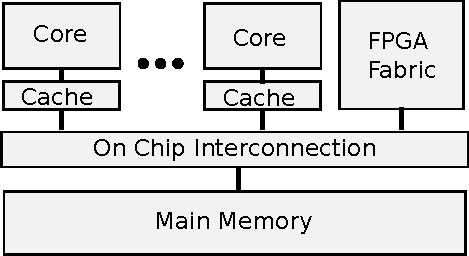
\includegraphics[width=0.5\linewidth]{system-context}}
\caption{System Context}
\label{fig:system-context}
\end{figure}

\subsection{HW/SW Codesign Using FPGA Accelerator}
This section introduces the basic HW/SW co-design flow using FPGA accelerator as given in Figure
\ref{fig:codesign}. Given a HLL program, computation intensive loops can be identified either
through a profiling or user directives. Then the loops are replaced with basic software
interfaces and the modified code goes through a conventional software compiling flow. Afterwards, the
binary code can be generated. While the loop is handled by the HLS tools. With user design constrain 
and platform specific parameters, the HLS tool translates the loop to either HDL or bitstrem depending 
on the user's choice. Finally, the binary code and bitstream are downloaded to the CPU+FPGA system.

\begin{figure}[H]
\center{\includegraphics[width=0.5\linewidth]{codesign}}
\caption{HW/SW Co-design Using FPGA Accelerator}
\label{fig:codesign}
\end{figure}

\subsection{SCGRA Based FPGA Accelerator}
Instead of compiling HLL program directly to FPGA, this work employs a SCGRA as an intermediate
layer for compiling. With this intermediate layer, the FPGA accelerator design could be
simplified as presented in Figure \ref{fig:scgra-accelerator}. It basically includes two parts: the
SCGRA and the on-chip buffer. SCGRA consists of an array of processing elements (PEs). They work
in lock-step with the assist of the operation scheduler assuming that all the data needed is
available in the on-chip buffer. While all the on chip buffer needs to do is to realize the
assumption of the SCGRA and to provide as large bandwidth as possible to the computation array. 
\begin{figure}[H]
\center{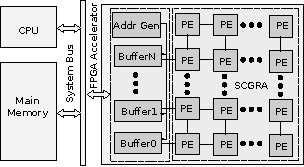
\includegraphics[width=0.7\linewidth]{scgra-acceleratorv2}}
\caption{FPGA Accelerator Based on A FPGA Overlay}
\label{fig:scgra-accelerator}
\end{figure}

\subsubsection{SCGRA}
This work employs a SCGRA as an intermediate layer to comile HLL loops to the target FPGA. 
Although the exact design of this SCGRA does not affect the design method, its implementation does have a
significant impact on the performance of the generated gateware.  

In this section, an instance of such a SCGRA design is thus presented to demonstrate the feasibility 
of producing high performance gateware. As shown in \ref{fig:pe}, a PE of this SCGRA is highly optimized 
for FPGA implementation, centering its design around a hard DSP block with the addition of
an instruction ROM and a multi-port data memory. In addition, a load/store path is implemented on
the PEs that are responsible for data I/O beyond the FPGA. Using this design as a template, it is
envisioned that a separate hardware design team, or the high-level compiler may be able to produce
similarly high-performance SCGRA that is optimized for the targeted application domain.

\begin{figure}[H]
\center{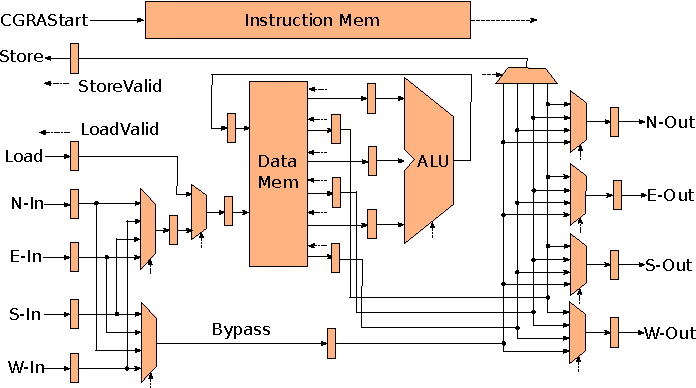
\includegraphics[width=0.9\linewidth]{pe}}
\caption{A Fully Pipelined PE Template}
\label{fig:pe}
\end{figure}

\subsubsection{On Chip Buffer}
On chip buffer bridges the system bus and the computation array. On the one hand, it loads/stores
data from/to the main memory through the system bus. On the other hand, it is connected to the
computation array and acts as an unified outside memory of the computation array. To achieve both
functionality, it is constructed as an interleaving memory using RAM blocks on FPGA. The
interleaving memory structure is a textbook design, but the difficult lies in how to decide the
interleaving parameters for target applications.

\section{Design Space Exploration}
The loop acceleration using FPGA is a HW/SW co-design and its performance is dramatically influenced by
a number of design parameters from hardware, software and the communication infrastructure. These
parameters construct a large design space and make the design space exploration extremely complex. 

\subsection{Design Space Overview}
To facilitate the design space exploration, this section presents a full design space exploration
overview based on the design flow as shown in Figure \ref{fig:design-space-overview}. The solid
lines with arrows briefly illustrate the design flow. Basically, the design flow takes HLL loop 
as well as target platform communication parameters as input. Then it goes through the software 
compilation, operation scheduling, application-specific SCGRA design and physical implementation. 

While the dashed lines with arrows show the possible design iterations using a straightforward
design space exploration. There are six possible design iterations locating at different levels of the design
flow and each design iteration has different design parameters included. 

The related design parameters of each design iteration is detailed in the 
table \ref{tab:detailed-design-parameter}. Note that the design 
parameters of the design iterations in upstream of the design flow naturally include the design parameters of the design
iterations in downstream of the design flow, so the design parameters in downstream of the design flow
will not be repeated in the upstream design iterations in the table. 

From the table, it can be seen
that loop unrolling factor stays at the first stage of the design flow, it has the most significant
impact on the loop acceleration. Following the loop unrolling, it is the on-chip buffer that has a group of
important design parameters. On the one hand, these parameters particularly the interleaving scheme determine 
the IO bandwidth of the SCGRA and have critical influence on the potential performance acceleration on SCGRA. 
On the other hand, the memory accessing order is also determined in this step and it influences the
memory accessing footprint and thus communication cost, which is one of the key design constrains of
the system. The rest design parameters such as the SGCRA design and the scheduling strategies mainly 
center the operation scheduler and have mutual influence on each other.

\begin{figure}[H]
\center{\includegraphics[width=0.8\linewidth]{design-space-overview}}
\caption{Design Space Overview}
\label{fig:design-space-overview}
\end{figure}

\begin{table}[H]
\caption{Detailed Design Parameters Involved in Different Design Iterations}
\label{tab:detailed-design-parameter}
\centering
\begin{tabular}{|p{0.8cm}|p{12cm}|}
\hline
1 & {Loop unrolling factors}\\

\hline
2 & {On-chip buffer size, interleaving scheme, data fetching scheme}\\

\hline
3 & {Primitive operations supported by the hardware infrastructure}\\

\hline
4 & {PE pipeline depth, local memory port number and allocation}\\

\hline
5 & {Topology of the computation array, array size}\\

\hline
6 & {Scheduling algorithm, scheduling strategies}\\

\hline
\end{tabular}
\end{table}

\subsection{Design Space Exploration Methods}
As mentioned in previous section, the system design space of compiling a HLL loop to a
tightly-coupled CPU+FPGA system is extremely large and a straightforward design 
will either result in long design iterations or less optimal design. Therefore, 
a systemic design space exploration will be of great importance for the
while design flow. 

Currently, I haven't got a complete solution to this problem, but I am trying to tackle it through a
both top-down and bottom-up analysis as detailed in the following steps. 

Step 1, Build a system model with appropriate assumption, and hopefully it may help find out the
most significant design parameters.

Step 2, Determine the design parameters that could be analyzed using local information so that the
design space could be scaled down. While the operation set basically depends on the computation 
involved in the loop and thus could be fixed at the beginning. 

Step 3, As DFG is the only input of the operation scheduler, it is possible to build a DFG analysis
algorithm such as machine learning. With sufficient training, the algorithm could provide an
estimated scheduling result without scheduling the DFG. This could help analyze the the optimal loop
unrolling.

%----------------------------------------------------------------------------------------
%	CONCLUSION
%----------------------------------------------------------------------------------------
\section{Current Progress}
This project follows Colin Yu Lin's work \cite{colinheart} which concentrated on building a SCGRA
with application-specific topology to provide an energy-efficient data flow computation. While it mainly
focuses on loop acceleration using a SCGRA based design flow on a CPU+FPGA system. To achieve this goal, 
I extended Colin's work and built a complete SCGRA based design flow to compile HLL program to 
FPGA. 

Afterwards, I did a few experiments on how to compile a loop to a SCGRA. Preliminary results
showed that fully unrolling is definitely not a reasonable solution, as it induces much longer compiling
time as well as larger hardware overhead with minor performance improvement. Partial loop
unrolling could solve this problem, but delicate loop unrolling algorithm is needed to find out the
optimal loop unrolling factor. 

Last but not the least, this work assumes a typical CPU and FPGA coexisting
system where communication between CPU and FPGA does cost a lot and it is nontrivial to the whole
system. In many applications with large data set, the communication cost may consume all the benefits 
brought by the kernel acceleration on FPGA and make the acceleration on FPGA useless. Therefore the
communication concern is taken in to consideration in the loop acceleration design and I worked on
Zedboard \cite{zedboard}, which is a commercial hybrid ARM+FPGA system, trying to move the whole SCGRA
work to it to verify the loop acceleration design method.

\subsection{SCGRA Based HLS Design Flow}
\ref{fig:design-flow} depicts an overview of the SCGRA based design methodology. As shown in the
diagram, the design methodology can be divided into two distinct parts. The first part, shown in the
top half of the figure, is expected to execute frequently. It should be executed every time a new
design iteration is required, a new debug cycle is started, or simply when a new application within
the same application domain is implemented. On the other hand, the second part of the design flow,
shown in the bottom half of the figure, is expected to execute infrequently, perhaps on a
per-application domain basis. Towards the end of the top half of the flow, the scheduling result is
merged with the pre-built bitstream from the bottom half to produce the final downloadable bitstream
for the target FPGA.
\begin{figure}[H]
\centering
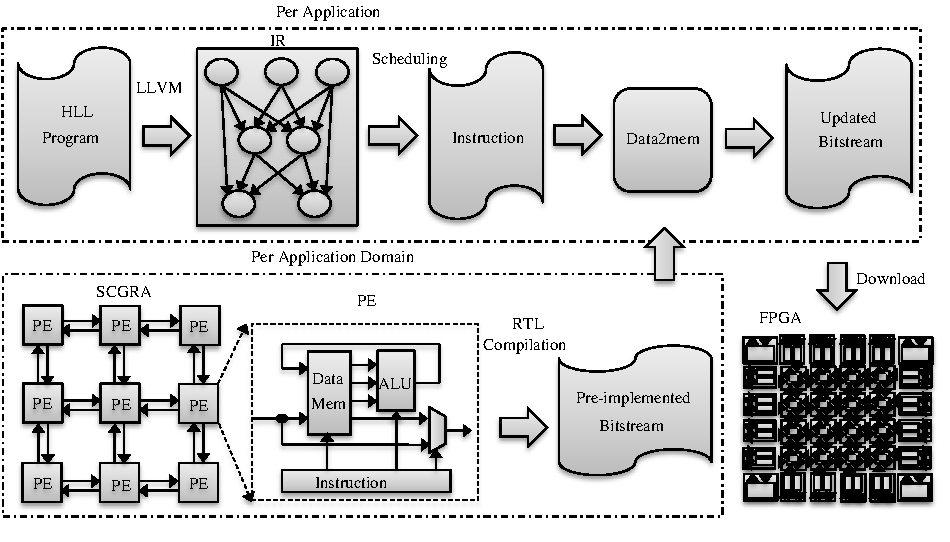
\includegraphics[width=14cm]{design-flow}
\caption{Overview of the SCGRA Based Design Methodology}
\label{fig:design-flow}
\end{figure}

\subsection{Loop Unrolling Exploration}
To analyze the influence of loop unrolling, three synthetic loop kernels are taken as examples. Each
kernel iterates 200 times, and thus the loop unrolling factor is limited to 1, 2, 4, ..., or 200 to
escape residual iterations. Figure \ref{fig:loop-unrolling} exhibits the influence of the loop unrolling 
on both performance and instruction memory which is the most concerned hardware resource. It is
clear that performance benefit gradually saturates with the increasing loop unrolling while the
instruction memory required increases a lot. Apparently, loop unrolling factor with near optimal
performance and moderate overhead exists between the fully unrolling and no unrolling.

As mentioned in the experiments, the loop unrolling factor is limited to a few numbers that can be
divided by the loop bound. Particularly, this can be a big trouble when the loop bound is a prime
number. A quick solution to this problem is simply leaving the residual loop iterations to software.
However, when there are two serial loops, this method will induce additional communication between
CPU and FPGA due to the residual loop iterations. To solve this problem, intermediate operations
that will be output at the last iteration of the SCGRA execution are also considered to be output 
during the scheduling. These intermediate operations are called breakpoints. They will not be stored
in outside memory unless the SCGRA goes to the last iteration. With this method, any loop unrolling
factor is allowed. Experiments as shown in Figure \ref{fig:any-loop-unrolling} proves that the 
performance penalty is ignorable.
\begin{figure}[H]
\centering
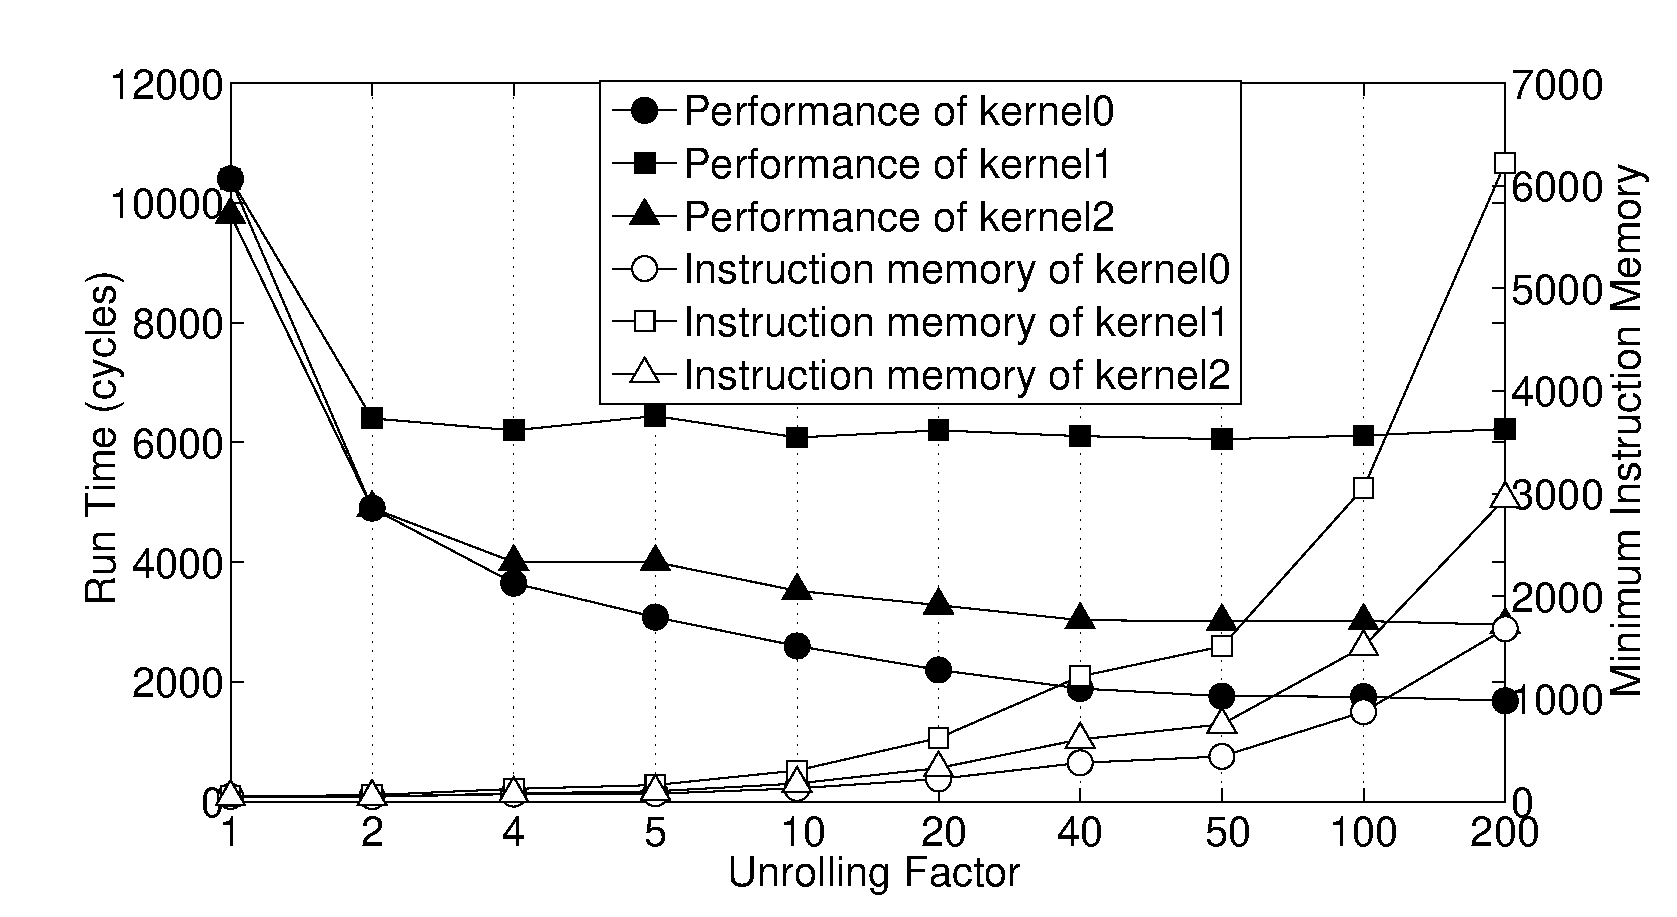
\includegraphics[width=10cm]{loop-unrolling}
\caption{Loop Unrolling Influence on Performance and Instruction Memory}
\label{fig:loop-unrolling}
\end{figure}

\begin{figure}[H]
\centering
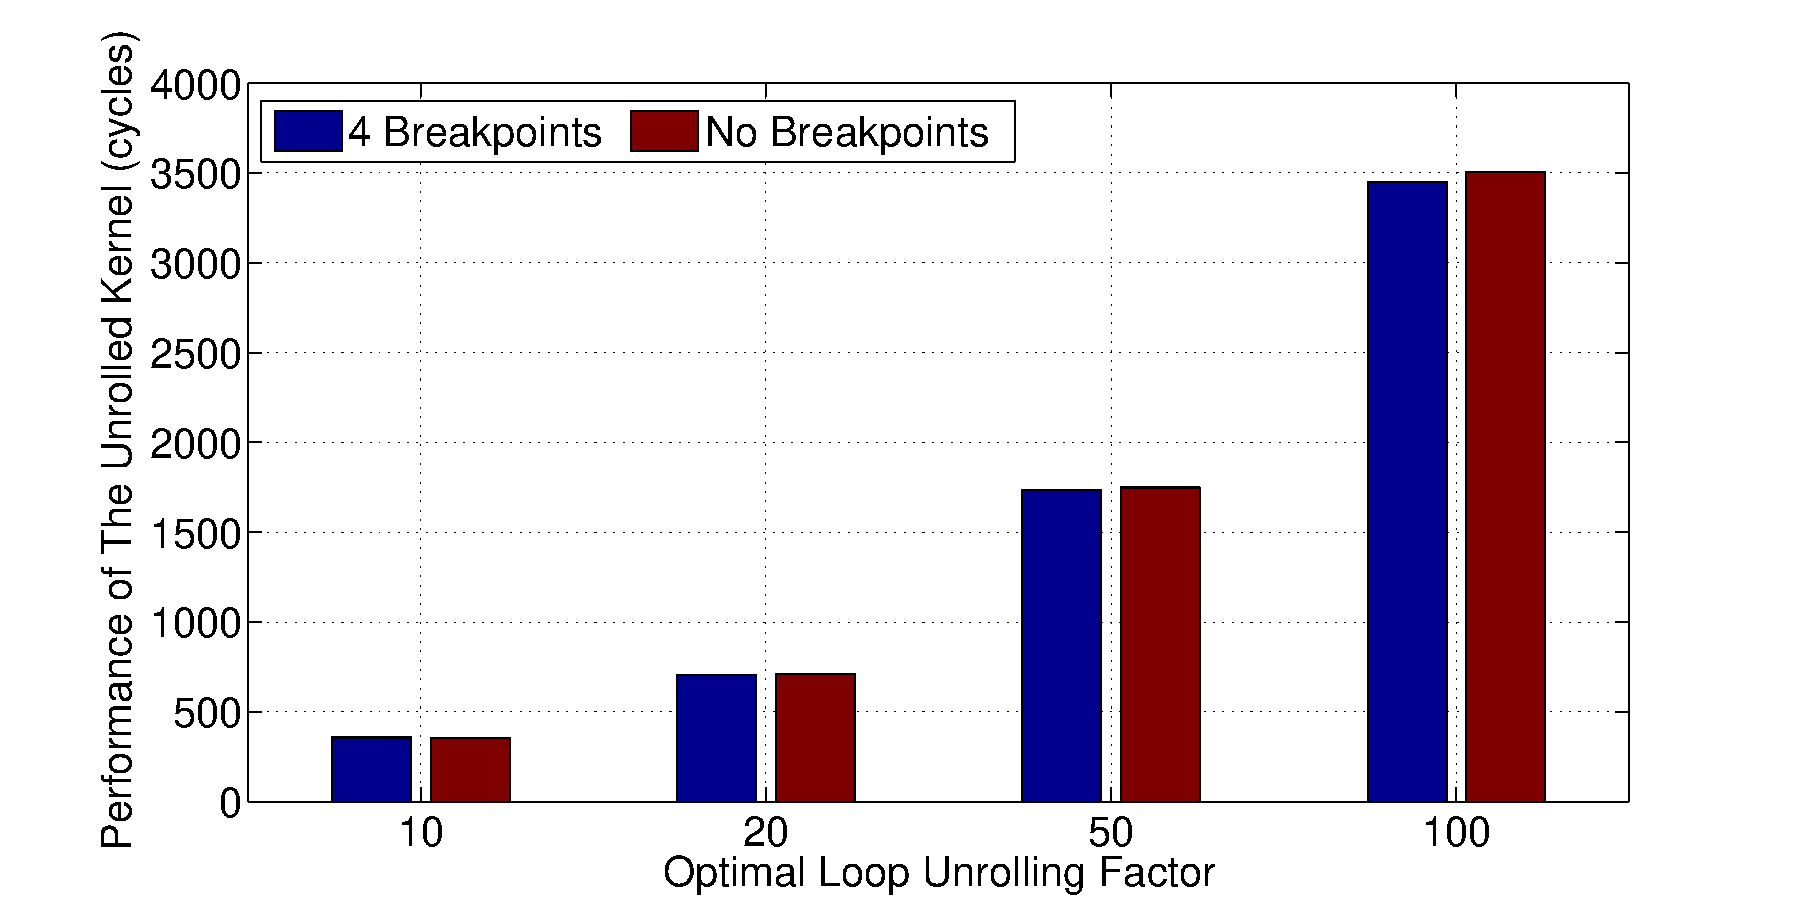
\includegraphics[width=8cm]{any-loop-unrolling}
\caption{Performance Of The Unrolled Loop Kernel With Breakpoints}
\label{fig:any-loop-unrolling}
\end{figure}

\subsection{SW/HW Communication on Zedboard}
Zedboard is a low-cost development board of the Zynq-7000 All programmable SoC. It integrates a
dual-core ARM Cortex-A9 based processing system (PS) and Xilinx programmable logic(PL) in a single
device. PS can be used for complex software as well as OS while PL can be used as an
accelerator to offload parallel computation of PS. To PL and PS co-design, it provides
a few ways of communication between PL and PS including accelerator coherence port (ACP), Central
DMA (CDMA), Normal DMA, and Video DMA (VDMA). ACP allows the PL to access the cache hierarchy and thus provides the
lowest communication latency. DMA and CDMA are similar and they are used to facilitate a group of
consecutive data transmission. The main difference is that DMA is shared by PS and PL while CDMA can only be used by PL.
VDMA is specially optimized for video application.

Since I am trying to accelerate loops in a HLL program and the communication between PL and PS may
vary, DMA is adopted as the default way to move data from/to main memory.(CDMA is actually a better
choice in terms of the performance, however, it is implemented on PL and consumes around 30\% of
the hardware resources.) A software centric PL/PS communication demo using the DMA has already been 
implemented on this board. Basically, software moves data to the shared memory between PL and PS.
When the data transmission is done, hardware takes over the shared memory and starts computation.
When hardware completes, it issues an interruption. Then software starts to collect the results at
pre-allocated address.

\section{Conclusion} 
Compiling loops with large data parallelism to FPGA accelerator and the rest program to GPP makes best use of
both advantages of CPU and FPGA. While FPGA accelerator has a large design space and the design
space exploration using either RTL or HLS tools is extremely time consuming. To overcome the
challenge, this project adopts the SCGRA based HLS design method to develop the loop accelerator.
Instead of simply concentrating on the loop kernel acceleration, this work takes the whole loop as
well as the hardware/sofware communication into consideration and aims to propose a complete design
space exploration method for loop acceleration on a tightly-coupled CPU+FPGA system. 

%----------------------------------------------------------------------------------------
%	BIBLIOGRAPHY
%----------------------------------------------------------------------------------------
\bibliographystyle{plain}
\bibliography{refs}
%----------------------------------------------------------------------------------------

\end{document}
